\section{Storage solutions}

During the 80s and 90s, data was mainly produced by humans.
However, in contemporary times, machines generate data at an unprecedented pace.

Various forms of media such as images, videos, audios, and social media platforms have emerged as significant sources of big data.
Moreover, the widespread deployment of sensors, surveillance cameras, digital medical imaging devices, and other technologies has further accelerated the accumulation of data.
This data deluge is further augmented by the integration of Industry 4.0 technologies and artificial intelligence, ushering in a new era of data-centricity and innovation.

The trend favors a centralized storage approach, which offers several advantages:
By limiting redundant data, it streamlines storage efficiency.
Automation of replication and backup processes ensures data reliability and security.
This centralized model ultimately leads to reduced management costs.

The current trend leans towards favoring a centralized storage strategy. 
This approach helps in minimizing redundant data, automating replication and backup processes, and ultimately reducing management costs.

HDDs have long dominated the storage technology landscape, characterized by magnetic disks with mechanical interactions.
However, recent technological advancements have introduced SSDs, which differ significantly. 
SSDs have no mechanical or moving parts and are constructed using transistors, specifically NAND flash-based devices.
Furthermore, NVMe (Non-Volatile Memory Express) has emerged as the latest industry-standard for running PCIe SSDs. 
Despite these innovations, tapes persist as a reliable storage solution unlikely to fade away.

Certain large storage servers employ SSDs as caches for multiple HDDs. 
Similarly, some latest-generation main boards integrate a small SSD with a larger HDD to enhance disk speed. 
Additionally, certain HDD manufacturers produce Solid State Hybrid Disks (SSHDs) that combine a small SSD with a large HDD within a single unit.

\subsection{Hard disk drive}
In the view of an operating system, disks are perceived as a compilation of data blocks capable of independent reading or writing. 
To facilitate their organization and management, each block is assigned a unique numerical address known as the Logical Block Address (LBA). 
Usually, the operating system groups these blocks into clusters, which serve as the smallest unit that the OS can read from or write to on a disk. 
Cluster sizes typically vary from one disk sector (512 bytes) to 128 sectors (64 kilobytes).
\begin{figure}[H]
    \centering
    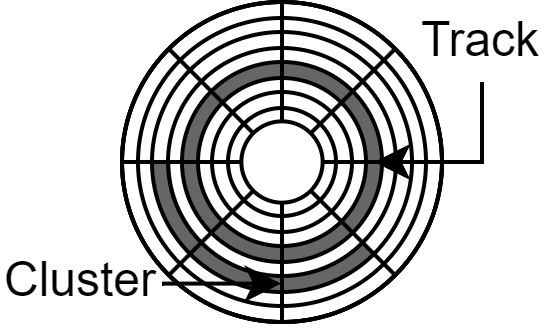
\includegraphics[width=0.4\linewidth]{images/hdd.png}
    \caption{Hard disk drive structure}
\end{figure}
Clusters encompass two crucial components:
\begin{enumerate}
    \item \textit{File data}: this refers to the actual content stored within files.
    \item \textit{Metadata}: this includes essential information necessary for supporting the file system, which consists of:
        \begin{itemize}
            \item File names.
            \item Directory structures and symbolic links.
            \item File size and file type.
            \item Creation, modification, and last access dates.
            \item Security information such as owners, access lists, and encryption details.
            \item Links directing to the Logical Block Address (LBA) where the file content is located on the disk.
        \end{itemize}
\end{enumerate}
Hence, the disk can harbor various types of clusters:
\begin{itemize}
    \item \textit{Fixed-position metadata}: reserved to bootstrap the entire file system.
    \item \textit{Variable-position metadata}: used to store the folder structure.
    \item \textit{File data}: housing the actual content of files.
    \item \textit{Unused space}: available to accommodate new files and folders.
\end{itemize}











\subsection{Solid state drive}

















